\documentclass{article}

\usepackage{ocencfd}

\title{Speech Recognition Based on Digital Spectrum Analysis and Template Matching} % Sets article title
\author{Amr Ramadan} % Sets authors name
\authorID{ARamadan} %Link to your profile ID.
\documentID{template} %Should be alphanumeric identifier
\fileInclude{} %Names of file to attach
\date{\today} % Sets date for publication as date compiled

% The preamble ends with the command \begin{document}
\begin{document} % All begin commands must be paired with an end command somewhere

	\maketitle % creates title using information in preamble (title, author, date)
    
	%New section is created
	\section{Introduction}
	%Plain text is just written directly in this document like this:
% 	This is a template. You can make references to things like \citep{latexsource}, which will show up in the bibliography (\sectref{bibsect}.)

    In this approach we will be receiving the voice commands from the user, analyze the input, in real time, into its frequency spectrum then project this spectrum on specific frequency bands and compare the magnitude to these projections with pre-stored templates to check the level of similarity and ,eventually, decide whether the input represents a good match or not.

% 	%New section about equations
% 	\section{Equations}
% 	Here is an inline equation: \ieq{F=ma}. Below is a block equation which we can label as \eqref{example_eqn}.

% 	\begin{equation} 
% 		\label{example_eqn}
% 		a^2+b^2=c^2
% 	\end{equation}

% 	%New section about tables and figures
% 	\section{Figures and tables}
% 	\figref{figtest} is an example figure. 

% 	\begin{figure}[h!]
%   		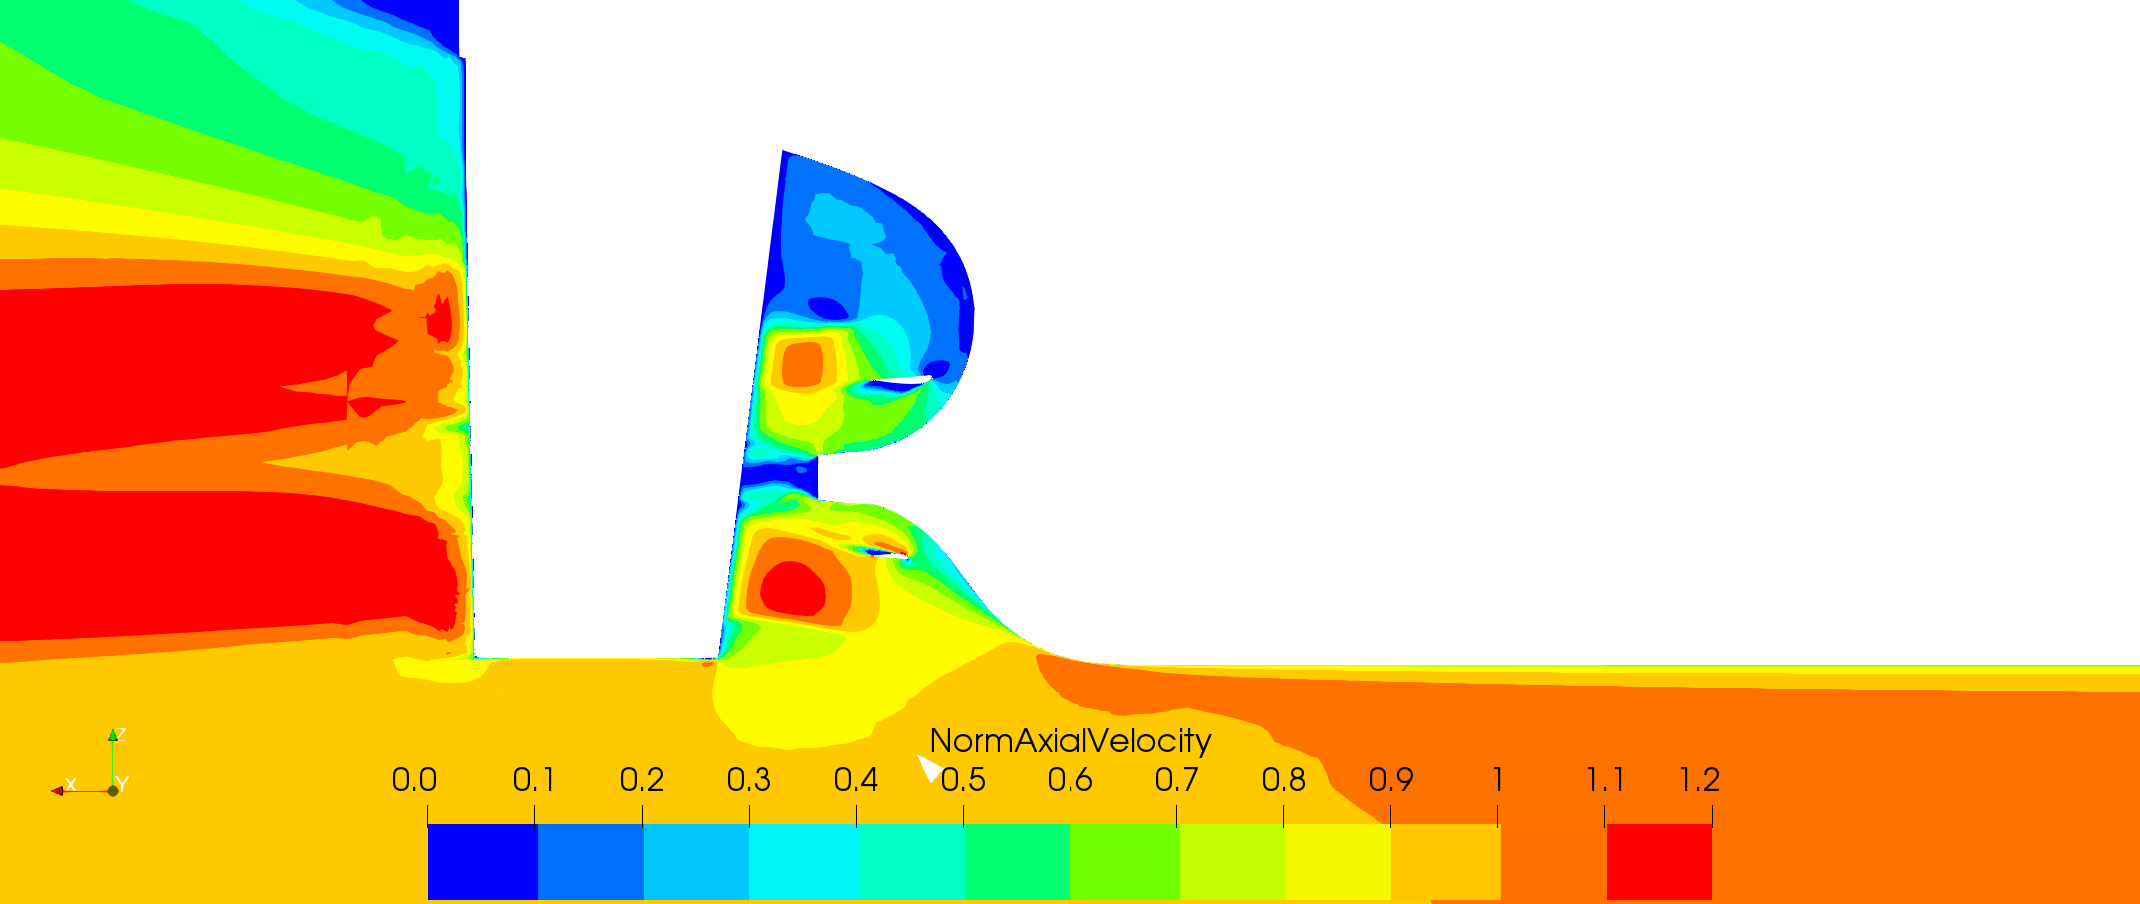
\includegraphics[width=\linewidth]{images/example.png}
%   		\caption{An example image.}
%   		\label{figtest}
% 	\end{figure}

 %%%%%%%%%%%%%%%%%%%% Required Materials %%%%%%%%%%%%%%%%%%%
    
    \section{Required Materials}
    
% 	\tableref{tabletest} 

	\begin{table}[h!]
		\caption{Required Materials.}
		\label{tabletest}
		\begin{center}
  			\begin{tabularx}{\textwidth}{ X X }
    				\toprule
    				Item & Description \\ 
    				\midrule
    				ESP32 Development Board & The main controller \\ 
    				
    				Microphone  & Main input device \\ 
    				
    				Mic. Amplifier circuit & Prepares the input audio for processing \\ 
    				
    				Push Buttons & Input control signals \\
    				
    				Breadboard x2 & Prototyping connections\\
    				
    				\bottomrule
  			\end{tabularx}
		\end{center}
	\end{table}
	
	
%%%%%%%%%%%%%%%%%%%%%% Methodology %%%%%%%%%%%%%%%%%%%%%%%%
	
	\section{Methodology}
	
	\subsection{Template creation}
	\label{subsec:template creation}
	Using the control buttons, the user initiates the template recording mode and records voice samples to be stored for later comparison. The voice command signal is received and amplified by the input amplifier circuit. The signal is then sampled with an adequate sampling rate using the built-in Analog To Digital converter (ADC) in the esp32 micro controller. The sampled signal is then passed throw a digital filter block of 7 to 10 filters (more details in \ref{subsec:digiatl filter block}). The signals' frequency spectrum is then analyzed and the magnitude response of the filter block is recorded.  
	
	\subsection{Audio Input}
	\label{subsec:audio input}
	The input is received from the user throw the Mic. and then preprocessed by the input amplifier circuit. Afterward, the built-in ADC in the esp32 is used to sample the input following the same procedures mentioned in \ref{subsec:template creation}. 
	
	\subsection{Template Comparison}
	\label{subsec:template comparison}
	Now, we are left with two pieces of data, namely, the template and the input sample. The template is stored permanently in a vector of floating point values representing the output of the digital filter block (more details in \ref{subsec:digiatl filter block}). The input signal components are stored temporarily after being analyzed by the filter block in a vector similar to that of the template. According to a predefined threshold, the input signal vector is compared to that of the input signal and a match is confirmed only if the similarity is higher than the threshold value (more details in \ref{subsec:detecting a match}). 
	
	
%%%%%%%%%%%%%%%%%%%% Implementation %%%%%%%%%%%%%%%%%%%%%	
	\section{Implementation}
	\label{sec:implementation}
	
	\subsection{Audio Amplifier Circuit}
	\label{subsec:audio amplifier circuit}
	[To be updated]
	
	\subsection{Digital Filter Block} 
	\label{subsec:digiatl filter block}
	
	The key part to achieve the desired results is have good resolution when analyzing the signal. A higher resolution can be obtained by dividing the frequency spectrum into more points. The proposed filter block works as follows: 
	
	\begin{enumerate}
	    \item The spectrum is divided into 7 to 10 critical points.
	    
	    \item These points are represented by the critical frequencies of the filters within the block.
	    
	    \item The filter block consists of:
	        \begin{itemize}
	             \item A low pass filter of critical frequency $f_{c0}$ which represents the lowest frequency band to be measured.
	             
	             \item Band pass filters of number $n$ and critical frequencies \{$f_{c1}$, $f_{c2}$, .. $f_{cn}$\}
	             
	             \item A high pass filter of critical frequency $f_{cn+1}$.
	        \end{itemize}
	        
        \item The frequency spectrum is defined by the critical frequencies $f_{c0}$ to $f_{cn+1}$, where $n$ is the number of filters within the block (in our case from 7 to 10 filters).
	    
	\end{enumerate}
	%%%%
	This design allows us to squeeze down the frequency spectrum of speech from its typical value ranging from $20~Hz$ to $20~KHz$ to a set of discrete bands ranging from $100~Hz$ to $1~KHz$. This specific range is chosen just for convenience as the human voice has its highest energy spectrum densities in the range below $1~KHz$ \ref{ref: paper}. The real question is why not add more filters? and the answer is quite simple, yet annoying, "We can't!". More filters mean more calculations, storage space, and more points to compare. Thus, demanding more computational power, faster clock cycles, and more storage space to accommodate the resulting vectors. 	\\\\
	The good news is that we haven't tested the esp32 for more than 10 filters yet, so, technically speaking, it can have more potential than the restrictions introduced in this proposal. The aim of these restrictions is to keep the hardware requirements as low as possible so that we can easily take the shift and implement the design on chips with lower capabilities than the esp32. \\\\
	An alternative design is to use second order Chebyshev band pass filter with all filters being band pass filters instead of having both lower, bass, and high pass filters \ref{ref:paper}.
	
	\subsection{Storing Templates}
	\label{subsec:storing templates}
	A challenging part is to save the templates permanently 
	as it happens that the esp32 has no Electronically Erasable Programmable Memory (EEPROM) on-board which means that we need to work around this by some means to make the templates persist after a power shutdown. We have to approaches in hand to tackle this problem, the first one is to, obviously, add an external memory chip to the system, and the other one is to explicitly use internal flash memory of the esp32. The later is achievable only if the size of the program is small enough for the template vectors to fit in without introducing any overflow conditions. [We need to experiment with using the internal flash memory to find out if it provides a good solution]  
	\subsection{Detecting a Match}		\label{subsec:detecting a match}
	Having template vectors stored and ready, we then need to compare the input vector in order to detect a successful match. Each item within the vector represents the magnitude response corresponding to one frequency band of the filter bank. For instance, if the filter bands are $100~Hz$, $200~Hz$, .., $1~KHz$, the vector has 10 items each representing the magnitude response of the convolution of the input signal and the corresponding filter. \\\\
	To decide if the how much the input signal matches the stored template, we had many methods in hand such as the Euclidean Norm,, and the Correlation Coefficient. [To be continued..]	
	

	%New section about code
	\section{Code}
	\label{sec:code}
	[To be updated]
% 	Below is some C++ code.
% 	\begin{lstlisting}[language=C++]
% tmp<fvVectorMatrix> tUEqn
% (
% 	fvm::div(phi, U)
% 	+ MRF.DDt(U)
% 	+ turbulence->divDevReff(U)
% 	==
% 	fvOptions(U)
% );
% \end{lstlisting}
   
	
% 	%Add bibliography at the end of document	
% 	\bibliography{template}
% 	\label{bibsect}

\section{Bibliography}
\label{sec:bibliography}
[To be updated]

\end{document} % This is the end of the document